%%%%%%%%%%%%%%%%%%%%%%%%%%%%%%%%%%%%%%%%%%%%%%%%%%%%%%%%%%%
%% Congratulations, you've made an excellent choice
%% of writing your Tampere University thesis using
%% the LaTeX system. This document attempts to be
%% as complete a template as possible to let you focus
%% in the most important part: the writing itself.
%% Thus the details regarding the visual appearance
%% and even structure have already been worked out
%% for you!
%%
%% I sincerely hope you will find this template useful
%% in completing your thesis project. I've tried to
%% add comments (followed by the % sign) to clarify
%% the structure and purpose of some of the commands.
%% Most of the magic happens in the file ./tauthesis,
%% which you are more than welcome to take a look at.
%% Just refrain from editing it in the most crucial
%% versions of the thesis!
%%
%% I wish you and your thesis project the best of luck!
%% If you've got any suggestions for improving this template,
%% please contact me via email at
%%
%% ville.koljonen (at) tuni.fi.
%%
%% Yours,
%%
%% Ville Koljonen
%% 16th May 2019
%%
%% PS. This template or its associated class file don't
%% come with a warranty. The content is provided as-is,
%% without even the implied promise of fitness to the
%% mentioned purpose. You, as the author of the thesis,
%% are responsible for the entire work, including the
%% provided material. No one else is liable to you for
%% any damage inflicted on you or your thesis were it
%% caused by using this template or not.
%%%%%%%%%%%%%%%%%%%%%%%%%%%%%%%%%%%%%%%%%%%%%%%%%%%%%%%%%%%

%%%%% PREAMBLE %%%%%

%%%%% Document class declaration.
% The possible optional arguments are
%finnish - thesis in Finnish (default)
%english - thesis in English
%numeric - citations in numeric style (default)
%authoryear - citations in author-year style
%draft - for faster non-final works, also skips images
%           (recommended, remove in the final version)
%programs - if you wish to display code snippets
% Example: \documentclass[english, authoryear]{tauthesis}
%          thesis in English with author-year citations
\documentclass[finnish, numeric]{tauthesis}  % draft -> kuvat ei lataudu

% The glossaries package throws a warning:
% No language module detected for 'Finnish'.
% You can safely ignore this. All other
% warnings should be taken care of!

%%%%% Your packages.
% Before adding packages, see if they can be found
% in ./tauthesis already. If you're not sure that
% you need a certain package, don't include it in
% the document! This can dramatically reduce
% compilation time.

\usepackage{todonotes}
% Add [disable]{todonotes} to remove todonotes and remove the setlength'

\usepackage{hyphenat}

\usepackage[final]{listings}
\usepackage{inconsolata}
\lstdefinestyle{sharpc}{
  language=[Sharp]C,
  showstringspaces=false,
  basicstyle=\footnotesize\ttfamily,
  numbers=left,
  stepnumber=2,
  numberstyle=\tiny,
  xleftmargin=0.6cm,
  xrightmargin=3.4pt,
  captionpos=b
}
\renewcommand{\lstlistingname}{Ohjelma}

\usepackage{graphicx}
\usepackage{pdfpages}

% Graphs
% \usepackage{pgfplots}
% \pgfplotsset{compat=1.15}

% Subfigures and wrapping text
% \usepackage{subcaption}

% Mathematics packages
\usepackage{amsmath, amssymb, amsthm}
%\usepackage{bm}

% The chemistry packages
% \usepackage{chemfig}
% \usepackage[version=4]{mhchem}

% Text hyperlinking
% \usepackage{hyperref}
% \hypersetup{hidelinks}

% (SI) unit handling
\usepackage{siunitx}

\sisetup{
    detect-all,
    math-sf=\mathrm,
    exponent-product=\cdot,
    output-decimal-marker={,} % for theses in FINNISH!
}

%%%%% Your commands.

% Print verbatim LaTeX commands
\newcommand{\verbcommand}[1]{\texttt{\textbackslash #1}}


% Basic theorems in Finnish and in English.
% Remove [chapter] if you wish a simply
% running enumeration.
% \newtheorem{lause}{Lause}[chapter]
% \newtheorem{theorem}[lause]{Theorem}

% \newtheorem{apulause}[lause]{Apulause}
% \newtheorem{lemma}[lause]{Lemma}

% Use these versions for individually
% enumerated lemmas
% \newtheorem{apulause}{Apulause}[chapter]
% \newtheorem{lemma}{Lemma}[chapter]

% Definition style
% \theoremstyle{definition}
% \newtheorem{maaritelma}{Määritelmä}[chapter]
% \newtheorem{definition}[maaritelma]{Definition}
% examples in this style

%%%%% Glossary information.

\loadglsentries[main]{tex/sanasto.tex}
\makeglossaries

%%%%% in citation information.

\addbibresource{tex/library.bib}

\begin{document}

%%%%% FRONT MATTER %%%%%

\frontmatter

%%%%% Thesis information and title page.

% The titles of the work. If there is no subtitle,
% leave the arguments empty. Pass the title in
% the primary language as the first argument
% and its translation to the secondary language
% as the second.
\title{Tarkkuuden parantaminen robotilla tarjoiltavien juomien kaatomäärissä}{Otsikko englanniksi}
\subtitle{Käytännön koe Drinkkirobotti-sovelluksella}{Alaotsikko englanniksi}

% The author name.
\author{Ossi Koski}

% The examiner information.
% If your work has multiple examiners, replace with
% \examiner[<label>]{<name> \\ <name>}
% where <label> is an appropriate (plural) label,
% e.g. Examiners or Tarkastajat, and <name>s are
% replaced by the examiner names, each on their
% separate line.
\examiner[Tarkastaja]{Lionel Hulttinen}

% The finishing date of the thesis (YYYY-MM-DD).
\finishdate{2021}{04}{13}

% The type of the thesis (e.g. Kandidaatintyö
% or Master of Science Thesis) in the primary
% and the secondary languages of the thesis.
\thesistype{Kandidaatintyö}{Bachelor of Science Thesis}

% The faculty and degree programme names in
% the primary and the secondary languages
% of the thesis.
\facultyname{Tekniikan ja luonnontieteiden tiedekunta}{Faculty of Engineering and Natural Sciences}
\programmename{Teknisten tieteiden kandidaatin tutkinto-ohjelma}{Bachelor's Programme in Engineering Sciences}

% The keywords to the thesis in the primary
% and the secondary languages of the thesis.
\keywords%
    {robotiikka}
    {robotics}

\maketitle

% Write the abstract(s) and the preface
% into a separate file for the sake of clarity.
% Pass the appropriate file name as the first
% argument to these commands. Put the \abstract
% in the primary language first and the
% \otherabstract in the secondary language second.
% Those who do not speak Finnish only need the
% first abstract. The second argument of
% the \preface command takes the place where
% the thesis was signed in.
\abstract{tex/tiivistelma.tex}
\otherabstract{tex/abstract.tex}
\preface{tex/alkusanat.tex}{Tampereella}

%%%%% Table of contents.

\tableofcontents

%%%%% Lists of figures, tables, listings and terms.

% Print the lists of figures and/or tables.
% Uncomment either of these commands as required.
% Both are optional, but if there are many important
% figures/tables, listing them may be a good idea.

% \listoffigures
% \listoftables
% \lstlistoflistings

% Print the glossary of terms.

\glossary

%%%%% MAIN MATTER %%%%%

\mainmatter

% Write each of the chapters of the thesis
% into a separate file for the sake of clarity.
% They can be \input as shown below. Give both
% the chapters and their files as descriptive
% names as possible.

\chapter{Johdanto}
\label{ch:johdanto}
Robotiikan käyttö maailmanlaajuisesti yleistyy koko ajan huomattavalla nopeudella. Roboteista tulee yhä älykkäämpiä ja taloudellisesti kannattavampia. Reilusti suurin osa roboteista on teollisuusrobotteja, jotka ovat kätketty tuotantolaitoksiin \cite{Heer2020}. Palvelurobotiikka kuitenkin kasvattaa myös osuuttaan, ja esimerkiksi robottiruohonleikkurit ja -imurit ovat aikaisempaan verrattuna suhteellisen tuttuja näkyjä kotitalouksissa. Myös esimerkiksi sote-aloilla palvelurobotteja käytetään jo melko laajalti \cite{Jyvaskylanyliopisto2018}. Yhä innovatiivisempia tapoja käyttää robotteja palvelualalla tulee esiin. Yksiä näistä ovat ravintola-alan sovellukset.

Juomia tarjoilevat robotit ovat toistaiseksi vielä melko uniikkeja. Juomien tarjoilu robotilla saattaa joissain tilanteissa nopeuttaa tarjoilua, mutta suurin myyntivaltti siinä on sen näyttävyys. Juomien automaattisessa tarjoilussa ongelmia aiheuttavat nesteen ominaisuudet. Usein robotit käyttävät hyväksi jonkinlaista juoma-automaattia \cite{Kelly2020} tai sitten pullot roikkuvat väärin päin esimerkiksi robotin päällä ja niissä on erityinen korkki, jota painamalla ja näin korkin venttiilin avaamalla robotti voi laskea pullosta juomaa \cite{Ro2016}. Näissä ratkaisuissa hyvä puoli on se, että nesteen virtaus tarjoiluastiaan on lähellä vakiota ja täten kokonaisjuomamäärä on helposti säädeltävissä. Tässä kandidaatintyössä käsitellään tapausta, jossa robotti kaataa juomaa pullosta mukiin. Tällöin juomankaatotehtävän voi antaa käytännössä mille tahansa robotille tarvitsematta juoma-automaatteja tai kokonaista robottisolua, jossa pullot roikkuvat robotin päällä. Pullosta kaataessa kuitenkin nesteen virtauksen ja pullon kallistuksen mukana tulevat muuttujat tekevät juomamäärän säätelystä hankalampaa.

Tässä kandidaatintyössä kerrotaan Pullonkaula ry:n Drinkkirobotti-sovelluksesta, ja siitä miten sillä on aikaisemmin toteutettu juomien kaato avonaisesta pullosta. Tämä tapa on sisältänyt ongelmia juuri kaatomäärän tarkkuuden suhteen, ja näitä ongelmia käsitellään alaluvussa \ref{ch:vanhan_ongelmat}. Tämän jälkeen kartoitetaan lyhyesti, millaisia ratkaisuja ongelmaan on kehitetty viime vuosina tehdyissä tutkimuksissa. Sen jälkeen valitaan ja perustellaan tässä työssä käytetty ratkaisu kaadon määrän ohjaamiseen. Lopuksi vertaillaan vanhan ja uuden kaatotavan käytössä saatuja tuloksia keskenään. Tämän työn pohjalta on mahdollista soveltaa kehitettyjä tekniikoita muihin samankaltaisiin sovelluksiin.


\chapter{Lähtökohdat}
\label{ch:lähtökohdat}

\section{Drinkkirobotti 5.0}
\label{ch:drinkkirobotti_5.0}
Drinkkirobotti 5.0 on Pullonkaula ry:n, eli Tampereen yliopistossa toimivan tuotantotekniikan ammattiainekerhon opiskelijoiden vapaa-ajalla tekemä projekti. Robottisolu koostuu Yaskawan HC-10-monitoimirobotin "You Teach Me"\hyp{}solusta ja sen ympärille rakennetuista baaritiskeistä. You Teach Me on Yaskawan valmiiksi valmisteltu opetuskäyttöön tarkoitettu robottisolukokonaisuus \cite{Yaskawa2017}. Baaritiskeissä on sisäpuolella pullohyllyt, ja kun robotilta tilataan juomaa, se hakee oikeat pullot hyllystä ja valmistaa niistä monikomponenttijuomia kaatamalla juomaa lasiin. Baaritiskillä on neljä paikkaa lasille. Robotilta juomien tilaaminen tapahtuu tabletille tehdyn käyttöliittymän avulla. Yaskawan HC-10 on yhteistyörobotti, eli se sisältää voima-antureita ja näiden avulla ihmisen ja robotin välinen yhteistyö on helpottunut. \cite{Pullonkaula2020}

\begin{figure}[h]
\begin{center}
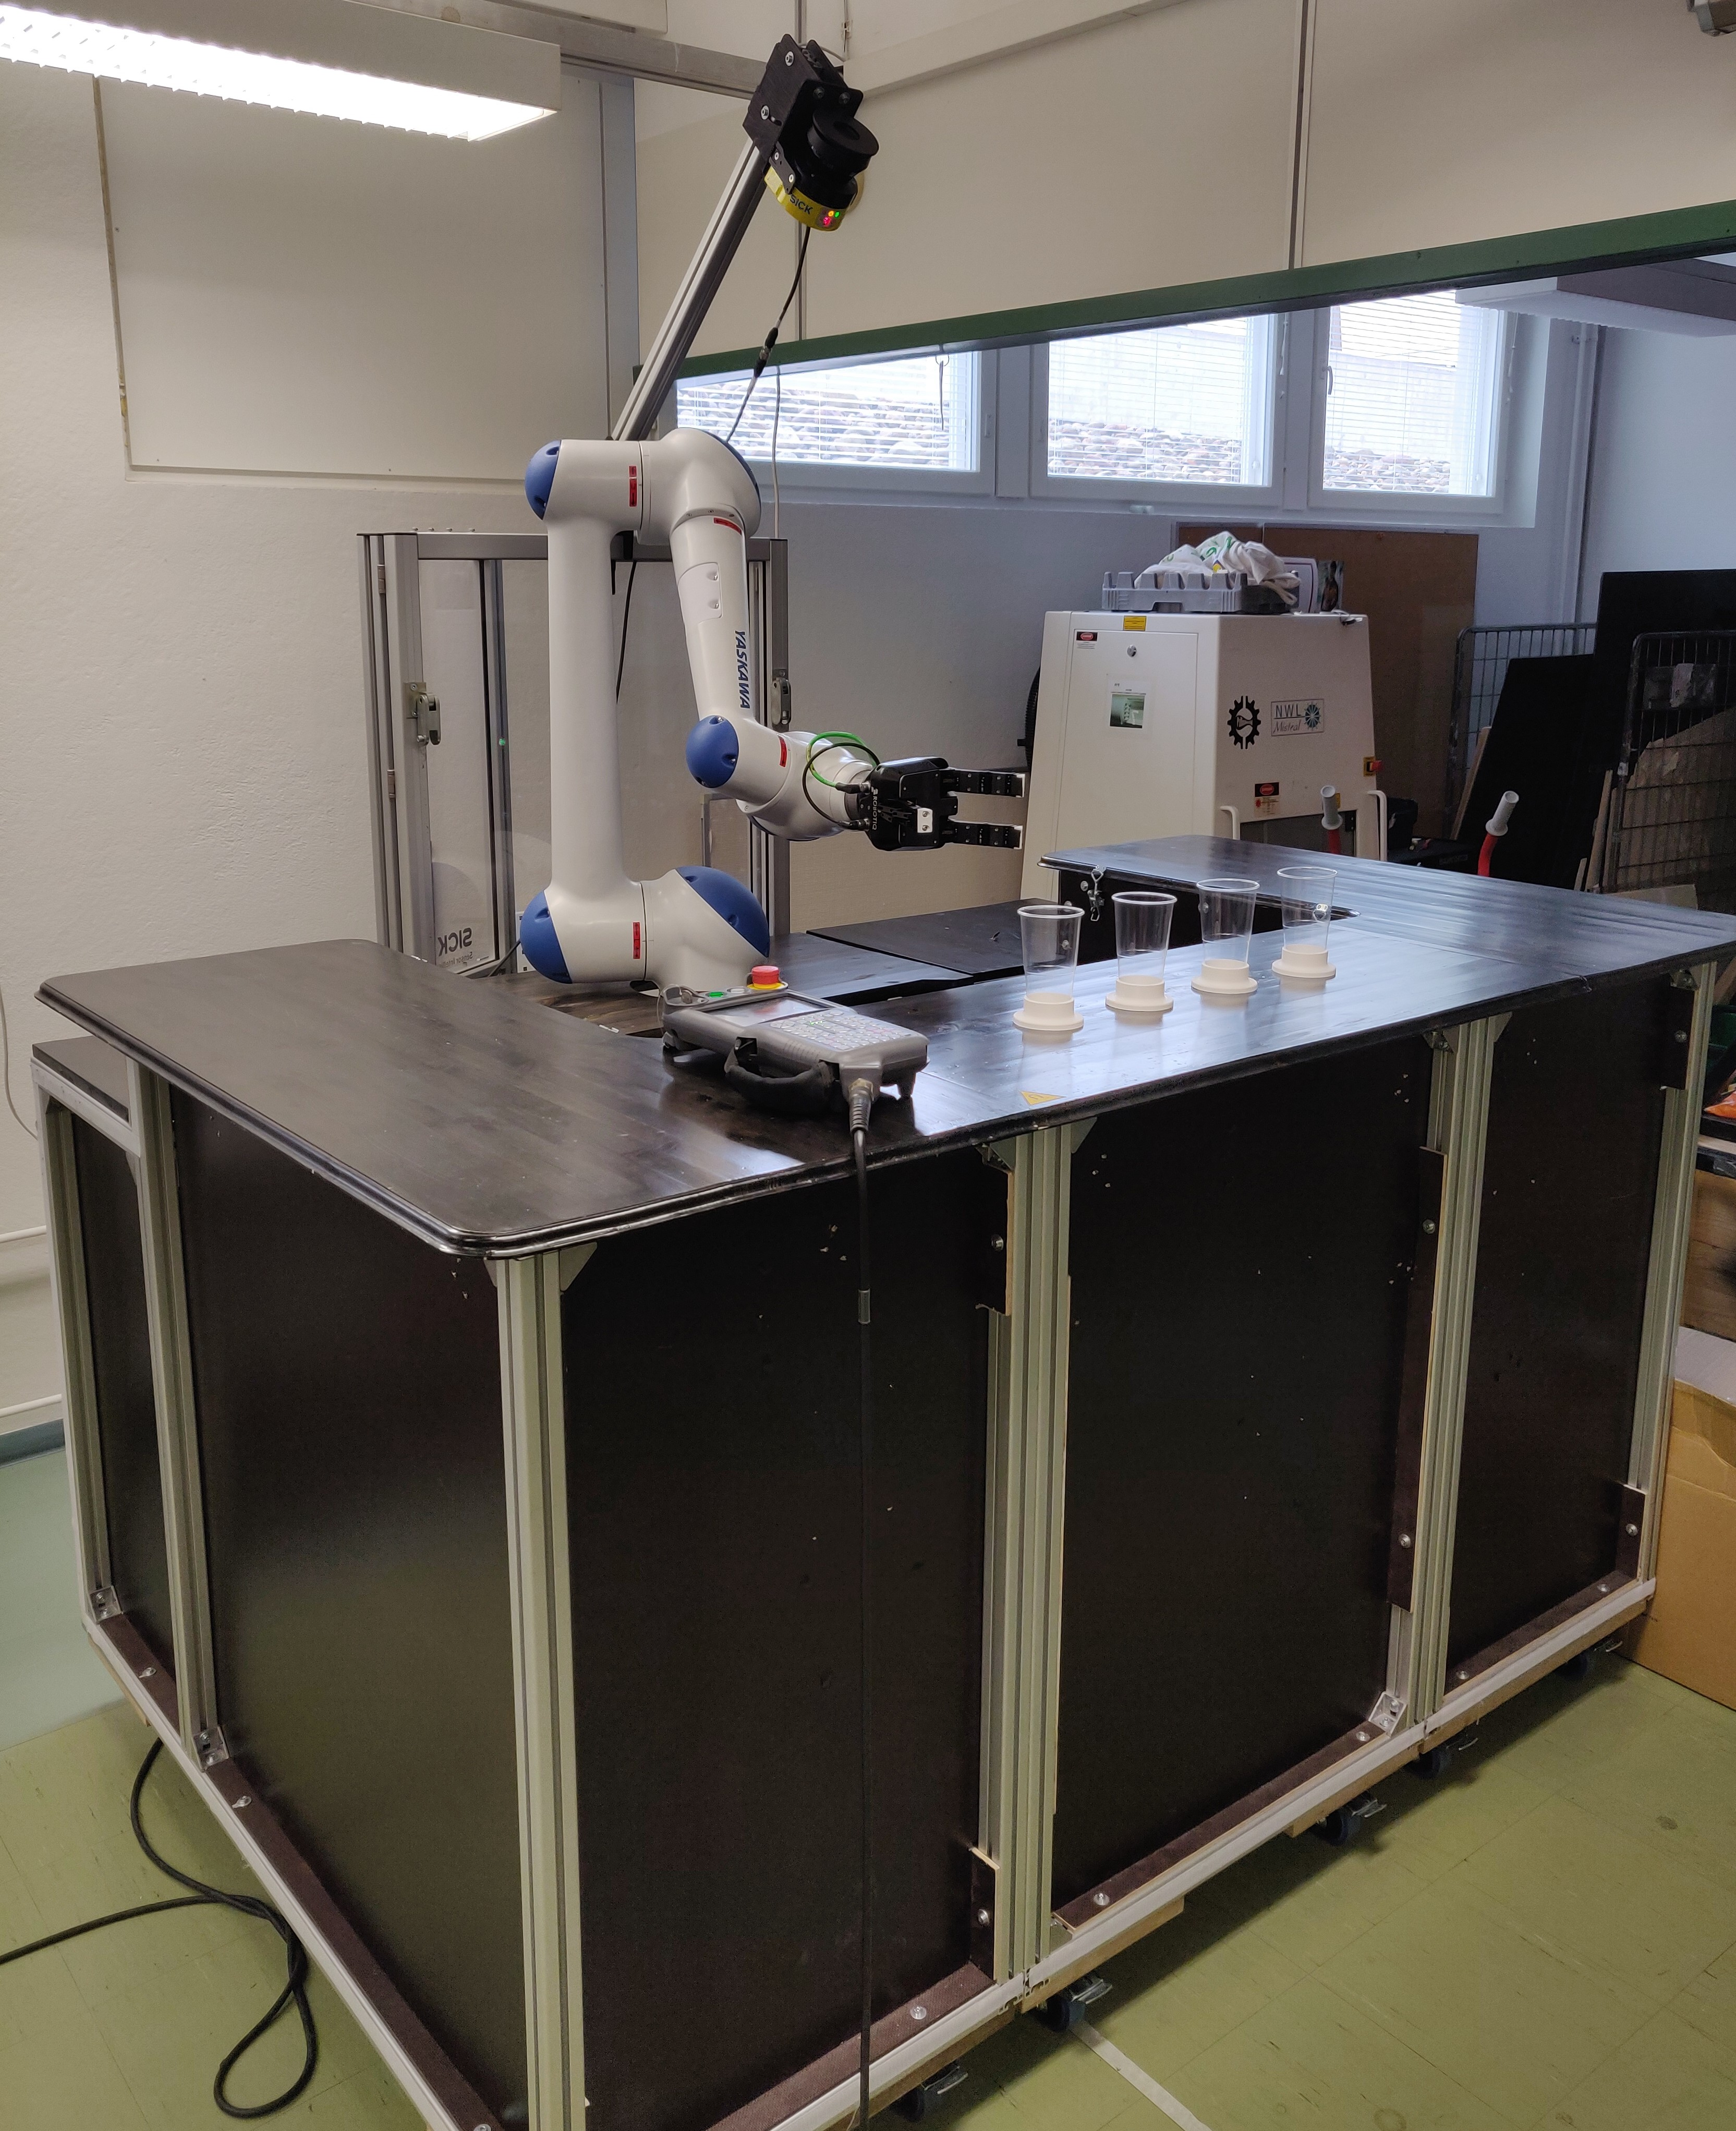
\includegraphics[scale=0.075]{img/drinkkirobotti.jpg}   % Scale 0.07 -> 0.075 -> Alla oleva teksti yhtä riviä alemmas.
\end{center}
\caption{Drinkkirobottisolu}
\label{fig:drinkkirobotti}
\end{figure}

Drinkkirobotin ohjelmisto koostuu useasta tasosta. Front end sisältää React.js:llä tehdyt käyttöliittymät operaattoria ja asiakasta varten. Operaattorinäkymästä voi esimerkiksi hallita robottisolun pullohyllyssä olevia pulloja lisäämällä tai poistamalla niitä ja valita robotin idle\hyp{}tilassa tekemiä liikkeitä. Asiakasnäkymästä voi selata tarjolla olevia juomia ja niiden sisältämiä komponentteja ja tilata juomia kerrallaan 1\hyp{}4 kappaletta. Back end toimii Node.js:llä ja se sisältää tiedon tarjolla olevista juomista ja niiden komponenteista sekä määristä. Siellä on myös reaaliaikainen tieto pullohyllyn tilanteesta, eli mitä pulloja hyllyssä on ja kuinka paljon juomaa missäkin pullossa on jäljellä. Kun operaattori lisää pullon, hän arvioi pullossa olevan juoman määrän ja merkitsee sen käyttöliittymään, joilloin juomamäärä välitetään back endille. Kun pullosta kaadetaan juomaa, back endiin päivittyy uusi tieto pullossa olevasta juomasta. Jos pullossa on liian vähän juomaa jäljellä minkään drinkin tekoon, robotti poistaa pullon hyllystä automaattisesti.

Itse robottikoodi on suhteellisen yksinkertaista. Siinä käytetään Yaskawan Inform \hyp{}ohjelmointikieltä, ja robottia ohjaa Yaskawan YRC-1000 -ohjausyksikkö. Robottikoodi sisältää "jobeja", jotka sisältävät robotin liikeratoja ja niiden parametrien määrittelyjä ja joissakin väleissä lyhyitä odotusaikoja. Robottisolun aivoina voidaan pitää sen bisneslogiikkatasoa. C\# -kielellä kirjoitettua logiikkaa pyörittää robottisolun sisällä oleva Rasperry Pi -tietokone. Logiikka ohjaa robottia kertomalla, mikä funktio, eli "job" milloinkin suoritetaan. Se siis käsittelee front endiltä saadut tilaukset ja päättää esimerkiksi mikä pullo haetaan ja mihin lasiin juomaa kaadetaan. Rasperry Pi ohjaa logiikan lisäksi robotin tarttujaa. Tarttujaa voidaan ohjata robottikoodista siihen tarkoitetuilla jobeilla, jolloin robottikoodi kutsuu Rasperry Pi:tä.

Uusimpana lisäyksenä robottisoluun on implementoitu vaaka, joka on niin sanotulla pullonvaihtopisteellä. Vaa'an toiminta on hyvä esimerkki robotti-bisneslogiikkarajapinnasta, sillä vaa'an voi kalibroida ja sen kullakin hetkellä näyttämää arvoa voi kysyä logiikan avulla. Tämän vaa'an avulla robotti tunnistaa, onko pullonvaihtopisteellä pulloa. Tätä käytetään esimerkiksi uuden pullon lisäämisessä: Kun robotti hakee uutta pulloa hyllyyn, niin se pysähtyy ensin pullonvaihtopisteen eteen. Jos vaaka kertoo, että pullonvaihtopiste on tyhjä, logiikka ei käske robottia hakemaan olematonta pulloa, vaan käskee sen odottamaan tietyn ajan. Robotti hakee pullon vasta, kun se lisätään pullonvaihtopisteelle. Tämän toiminnallisuuden avulla robotti ei siis vie olematonta pulloa hyllyyn, jolloin back endissä olisi tieto pullosta tietyllä kohdalla pullohyllyä, vaikka pulloa ei oikeasti ole. Samoin, jos robotti on poistamassa pulloa pullohyllystä, ei se vie sitä pullonvaihtopisteelle jos siellä on jo pullo. Näin robotti ei työnnä vanhaa pulloa vaihtopisteeltä alas, vaan odottaa että se poistetaan sieltä. Työn alla on myös ominaisuus, jossa logiikka kertoo back endille, miten paljon juomaa lisätyssä pullossa on, ja operaattorin tehtäväksi jää vain tarkistaa lukema, eikä itse arvioida lisättävässä pullossa olevaa juoman määrää.

\begin{figure}[h]
\begin{center}
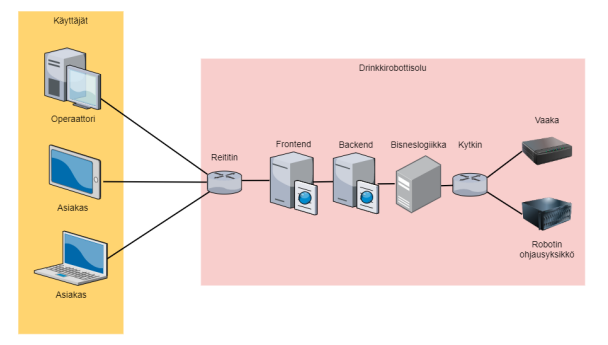
\includegraphics{img/rakenne_lowres.png}
\end{center}
\caption{Ohjelmistorakenne [lähde]}
\label{fig:rakenne}
\end{figure}

Vaaka koostuu HX711-mittakortista ja siihen kytketystä 5kg painoanturista, ja näitä ohjaa arduino-kirjastoja apuna käyttäen ohjelmoitu NodeMCU V3. Kommunikaatio logiikkaan toimii wlan-yhteydellä lähetettävillä UDP-paketeilla. Vaakaa pystyy siis siirtämään, ja niinpä tätä samaa vaakaa käytetään juomankaatosysteemin takaisinkytkentään, josta kerrotaan kappaleessa 3.


\section{Vanha kaatoratkaisu}
\label{ch:vanha_kaato}
Tässä alaluvussa käsitellään useamman vuoden käytössä ollutta ratkaisua juomien kaatamiseen Drinkkirobotilla. Ratkaisussa juomien kaadolle robottikoodissa on yksittäinen tehtäväohjelma, joka on esitetty alla ohjelmassa \ref{prog:POURDRINKS}.

\lstset{style=Yaskawatyyli}
\lstinputlisting[label={prog:POURDRINKS}, caption={POURDRINKS-tehtäväohjelma}]{code/POURDRINKS.txt}

Kaadon tarkkuutta tarkasteltaessa merkittävä osa tehtäväohjelmassa on ensimmäinen if-else-haara, joka alkaa ohjelman \ref{prog:POURDRINKS} riviltä 5. Se käsittelee kaadossa rivillä 24 käytetylle ajastimelle annetun arvon laskentaa. Haluttu kaadon määrä senttilitroina on asetettu muuttujaan I003. POURDRINKS-tehtäväohjelma laskee alussa ajan, jonka mukaan robotti kaataa juomaa. Kuten ohjelmasta \ref{prog:POURDRINKS} nähdään, kaadon aika sekunteina saadaan kaavalla
\begin{align}
   t = 60 \cdot V - 171 \mathrm{,}
\end{align}
jossa V on muuttuja I003 eli haluttu tilavuus senttilitroina. Kyseessä on lineaarinen yhtälö, jossa kulmakerroin 60 ja vakiotermi -171 on määritetty kokeellisesti kaatamalla eri määriä juomia. Ensimmäisen if-elsen tehtävä on myös tarkastaa, onko haluttu kaatomäärä alle kolme senttilitraa. Tätä pienemmillä määrillä yllä kuvattu lineaarinen funktio antaisi negatiivisen ajan. Niinpä kaikilla määrillä, jotka ovat alle kolme senttilitraa, kaatoajaksi on määritelty yksi sekunti.

Tehtäväohjelma toimii siis pääpiirteittäin siten, että robotti liikkuu kohteena olevan mukin kohdalle ja kallistaa pulloa. Kun pullo on kallistunut kaatoasentoon, käynnistyy ajastin, jonka kesto on määritelty muuttujaan I011.

Tämä tehtäväohjelma hoitaa kaadon useammalle mukille samalla, sillä siinä käytetään silmukkaa LABEL10- ja LABEL999-lippujen sekä muuttujien I004 ja I005 avulla. Muuttuja I005 on lasin numero, johon robotti sen hetkisellä iteraatiolla kaataa. Muuttuja I004 taas on haluttujen lasillisten määrä. Tehtäväohjelma CALCULATEPOUR laskee koordinaatit, joissa kohdemuki on ja tallettaa sen P-alkuisiin paikkamuuttujiin. Tässä se käyttää apuna muuttujaa I005. Mukipaikat ovat vaakasuorassa rivissä, joten siirryttäessä mukilta toiseen riittää vain lisätä robotin koordinaatiston x-koordinaattia mukien etäisyyden verran.


\section{Vanhan kaatoratkaisun ongelmat}
\label{ch:vanhan_ongelmat}
Edellisessä kappaleessa kuvattu ratkaisu on toiminut kohtalaisen hyvin useamman vuoden ottaen huomioon sen yksinkertaisuuden. Siinä on kuitenkin selkeitä heikkouksia. On selvää esimerkiksi, että alle kolmen senttilitran kaatoja tällä toteutuksella ei käytännössä voi tehdä. Tämä toteutus ei myöskään ota huomioon mitään muita muuttujia mitä juomien kaadossa voi olla halutun juomamäärän lisäksi. Tässä kappaleessa käydään läpi erilaisia ongelmia, joita vanhassa kaatoratkaisussa on ollut.

Eri muuttujien vaikutusta juoman kaatoon on yritetty vähentää käyttämällä aina samanlaisia pulloja, ja sen lisäksi pulloissa kaatonokkia. Tämä helpottaa myös kaatoliikkeen ohjelmointia robotille, kun pullosta tuleva juoman virtaus osuu mukiin helpommin. Virtaus on myös tasaisempi kaatonokkaa käytettäessä. Kaatonokassa on pieni korvausilmaputki, joka tasaa painetta pullon sisä- ja ulkopuolella. Kaatoja pullosta ilman kaatonokkaa ovat simuloineet Geiger et al. Simulaatiosta huomataan, miten normaalisti pullon suusta kaadettaessa ilman pitää virrata kaatoaukosta välillä sisäänpäin. Tämä aiheuttaa nesteen virtaukseen nykivää liikettä, jota ei kaatonokkaa käytettäessä tule korvausilmaputken ansiosta.

%\newpage

\begin{figure}[h]
\begin{center}
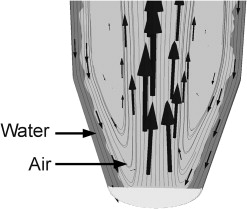
\includegraphics[scale=1.1]{img/Geiger et al. juoman virtaus.jpg}
\end{center}
\caption{Juoman virtaus \cite{Geiger2012}}
\label{fig:juomien_virtaus}
\end{figure}

Varsinkin kapeilla ulostuloputkilla ilmavirtaus juoman virtausta vastaan tekee juoman virtauksesta huomattavasti turbulenttisemman, mikä vaikuttaa juoman virtausnopeuteen. \cite{Geiger2012} Kapea ulostuloputki on siltä kannalta parempi, että sellaista käytettäessä robotin on paljon helpompi osua lasiin juomaa kaataessa, kun virtaus on kooltaan kapeampi.

\begin{figure}[h]
\begin{center}
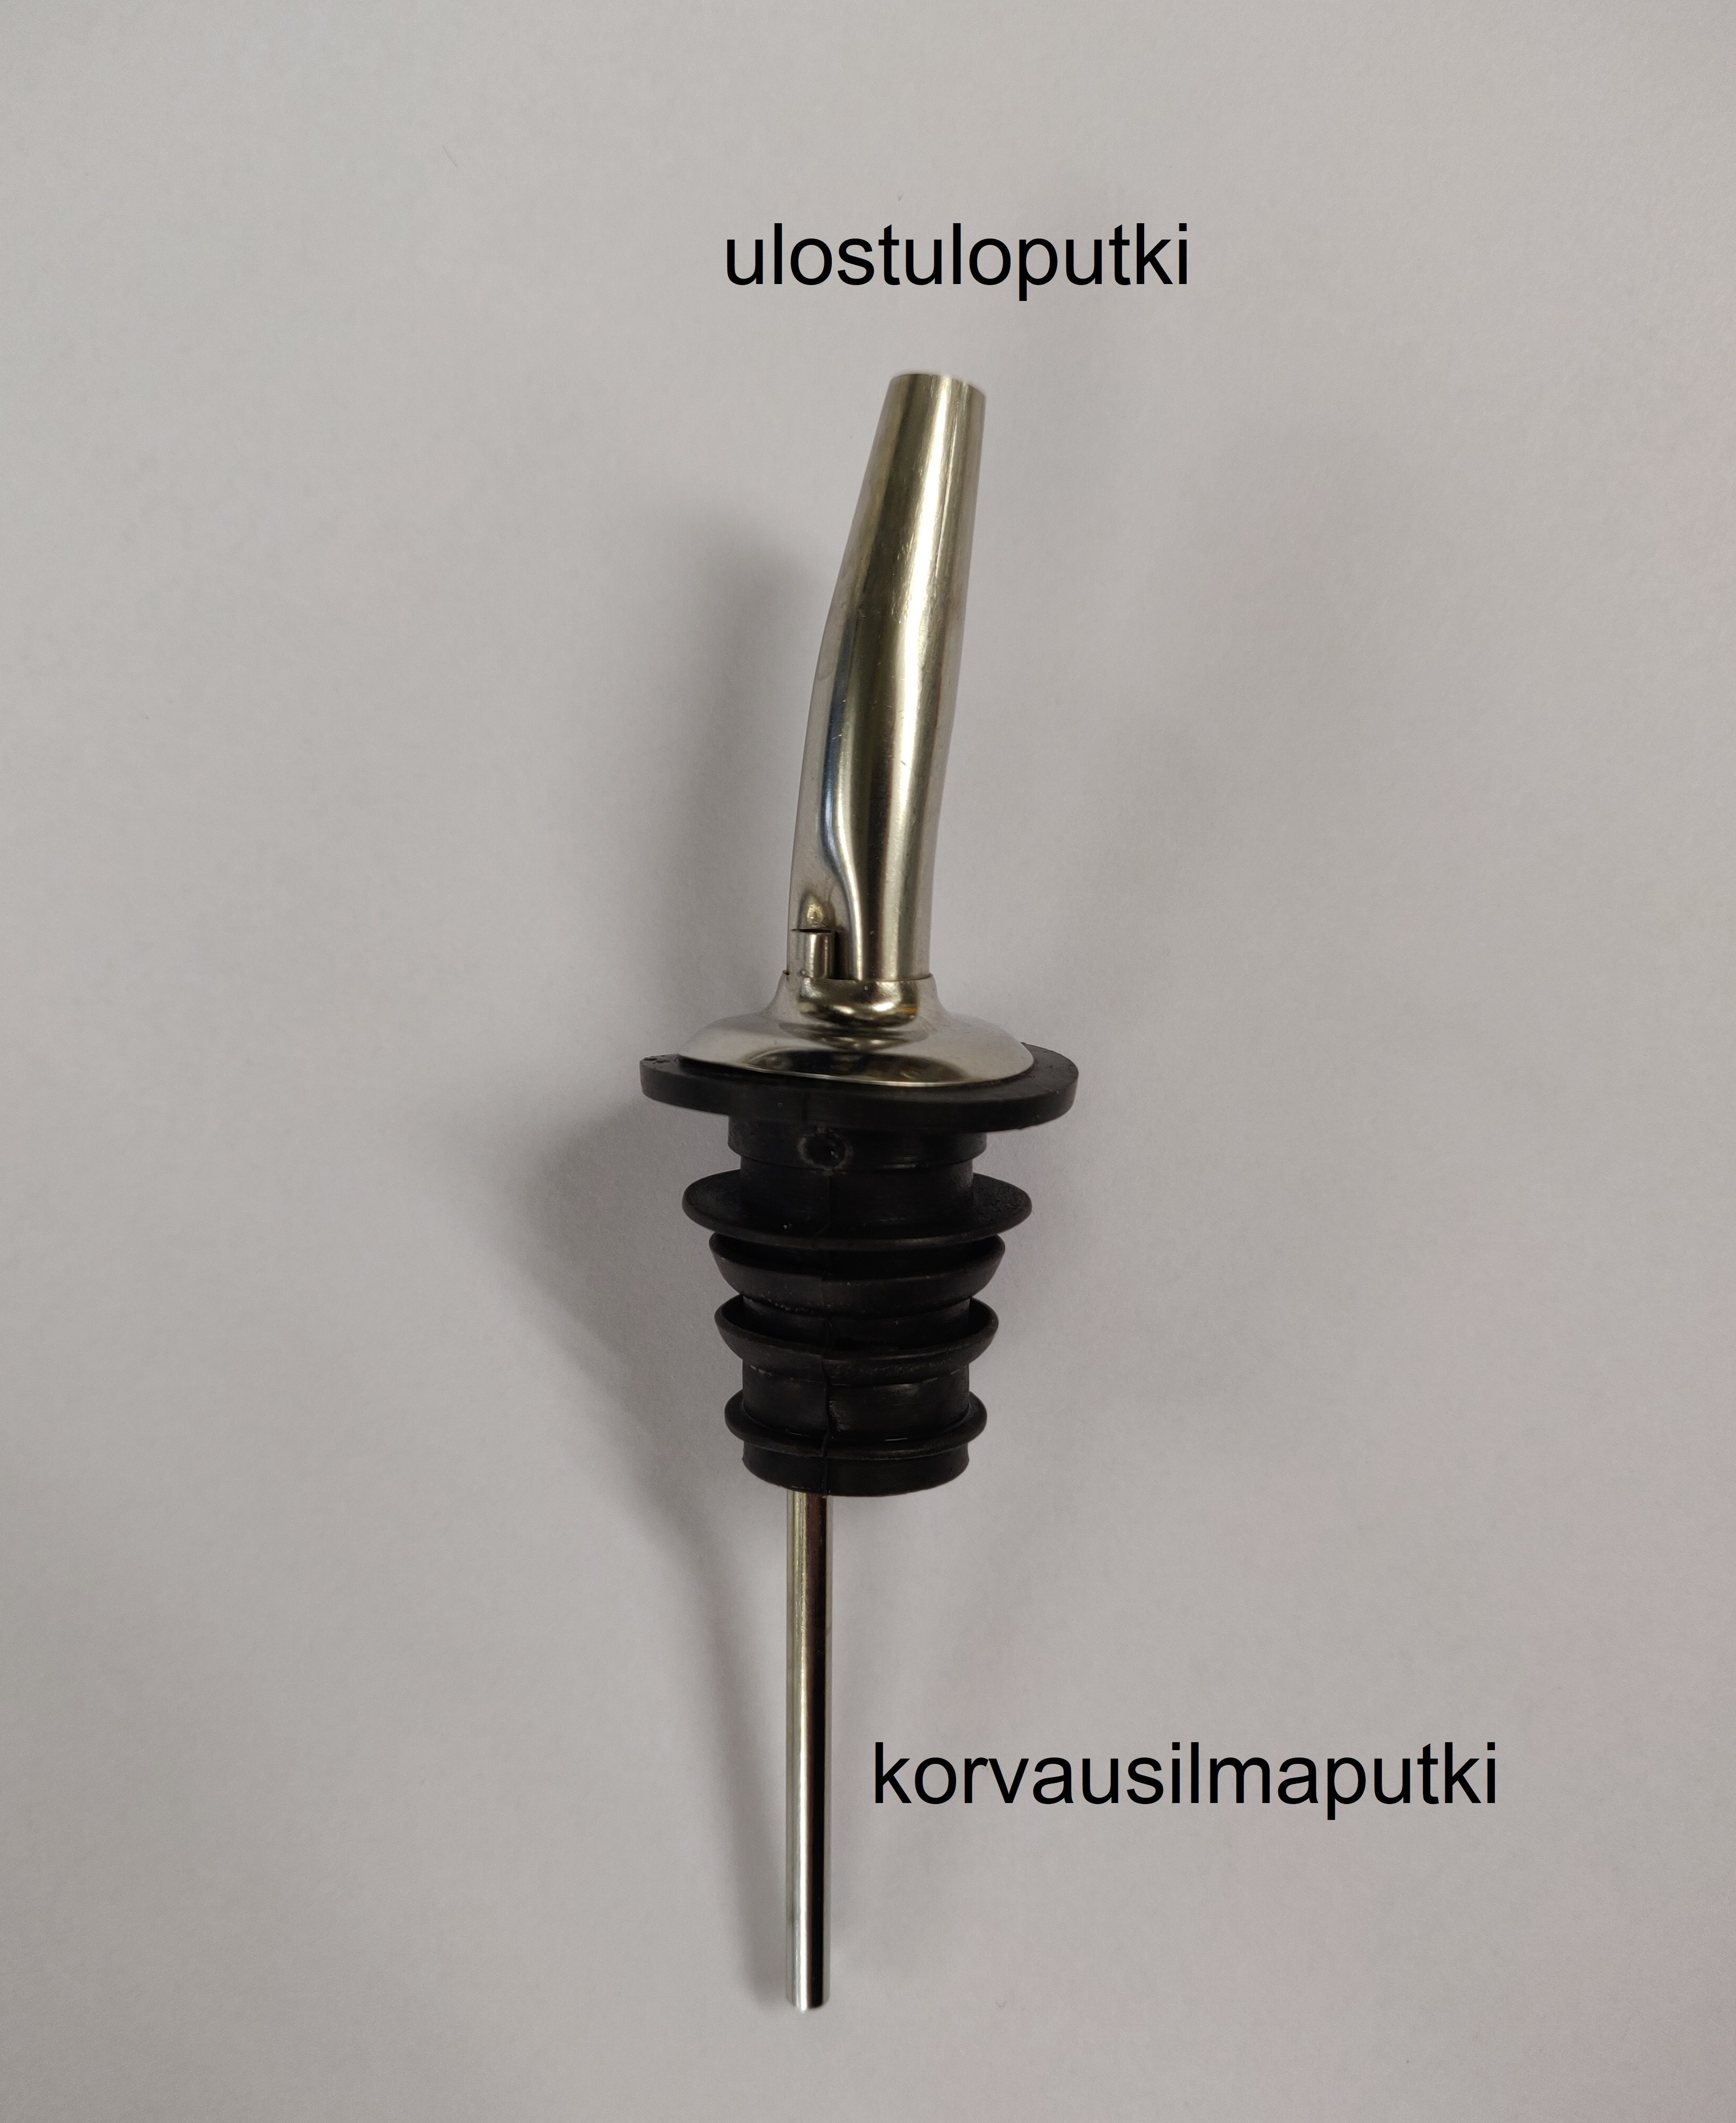
\includegraphics[scale=0.08]{img/kaatonokka.jpg}
\caption{Kaatonokka, johon on merkitty ulostuloputki ja korvausilmaputki}
\label{fig:kaatonokka}
\end{center}
\end{figure}

Juoman kaatamisessa robotilla on kuitenkin omat ongelmansa, vaikka käytössä olisikin kaatonokka. Suurin ongelmista tässä sovelluskohteessa on se, että korvausilmaputkeen saattaa mennä pisara nestettä. Näin pullon sisään ei tule korvausilmaa, ja kaatonokasta ei virtaa nestettä liian suuren paine-eron takia, vaikka pullo olisi kokonaan ylösalaisin. Tällaista tilannetta ei robotti ole osannut havaita. Sen takia asiakkaan lasi on jäänyt käytännössä tyhjäksi ja juomatilaus on jouduttu tekemään uudelleen. Tavoite uudelle kaatoratkaisulle on tällaisen tilanteen tunnistaminen ja siitä palautuminen.

Juomien kaatoon muuttujia tuo huomattavasti lisää myös se, millaista juomaa kaadetaan. Veden, mehujen ja muiden kuohumattomien ja viskositeetiltään samankaltaisten juomien kaataminen onnistuu vielä melko hyvin lineaarisen funktion mukaan, mutta ongelmia alkaa tulla varsinkin kuohuvien juomien kanssa. Tällöin saman lineaarisen funktion käyttö ei enää toimi, sillä esimerkiksi kuplat aiheuttavat turbulenssia kaadon aikana. Vettä paljon suuremman viskositeetin omaavat nesteet ovat dynamiikaltaan erilaisia, sillä korkeampi viskositeetti pienentää virtausnopeutta \cite{Lumen2021}. Tämän takia niiden kaataminen ei myöskään onnistuisi vanhalla toteutuksella.

Pullossa jäljellä oleva juoman määrä vaikuttaa kaadossa siihen, miten paljon juomaa virtaa pullosta. Kun pullo on täysin kaatoasennossa, juomaa virtaa vakiomäärä, mutta ero tulee kallistus- ja suoristusliikkeiden aikana. Kun pullo on täynnä, juomaa alkaa virtaamaan pullosta paljon pienemmällä kallistuskulmalla kuin siinä tapauksessa, jos pullossa on enää vähän juomaa jäljellä. Tämän vaikutusta kaatomäärään on pyritty pienentämään tekemällä kallistus- ja suoristusliikkeet nopeasti.

Juomien kaatomäärän tarkkuus on tärkeää monestakin syystä. Varsinkin jos tarjoiltava juoma sisältää alkoholia, vaikuttaa asiaan Suomen lainsäädäntö ja alkoholilaki. Alkoholilaissa on kirjattu alkoholijuomien perusannokset: ``Väkevien alkoholijuomien perusannos on 4 senttilitraa, enemmän kuin 15 tilavuusprosenttia etyylialkoholia sisältävän miedon alkoholijuoman perusannos on 8 senttilitraa, enemmän kuin 8 mutta enintään 15 tilavuusprosenttia sisältävän miedon alkoholijuoman perusannos on 12 senttilitraa ja muun miedon alkoholijuoman perusannos on 33 senttilitraa.'' \cite{Finlex} Lakisääteisyyden lisäksi on monta komponenttia sisältävissä juomasekoituksissa maun kannalta tärkeää, että komponentteja juomasekoituksessa oikea määrä. Usein asiakkaat ovat myös kiinnostuneet siitä, onko robotti kaatanut tasaisesti ja näin he vertailevat juomalaseja keskenään.

Asiakkaan näkökulman lisäksi ongelmat kaatojen määrässä kertautuvat, kun robotin back end saa väärää tietoa pulloista kaadetuista määristä. Jos robottia kutsutaan kaatamaan esimerkiksi kymmenen senttilitraa juomaa, ja juomaa kaatuukin senttilitra liikaa, niin back end laskee pullosta lähteneen silti kymmenen senttilitraa. Kun tämä tapahtuu tarpeeksi monta kertaa, niin back endin tieto pulloissa jäljellä olevista juomista ei pidä enää paikkaansa. Pahimmillaan back endissä voi olla tieto, että pullosta riittäisi juomaa vielä yhteen lasilliseen, mutta todellisuudessa kyseinen pullo on lähes tyhjä. Tällöin jää operaattorin vastuulle huomata, että juoma pullossa ei riitä. Näin voidaan taas joutua tilanteeseen, jossa asiakas tilaa juomaa, mutta saakin vain tyhjän lasin.

Robotin logiikassa on ominaisuus, joka tarkistaa, onko pullossa liian vähän juomaa jäljellä ja se kutsuu suoraan pullon poistoa solusta. Jotta ei päädyttäisi tilanteeseen, missä lähes tyhjästä pullosta yritetään tarjoilla juomaa, on jouduttu määrittelemään palautettavan pullon jäljellä olevaksi juomamäärän rajaksi melko korkea määrä. Tällöin robotti poistaa solusta pulloja, jossa juomaa olisi vielä tarpeeksi, koska ei haluta että joudutaan tilanteeseen, joka haittaa asiakasta. Uudella kaatoratkaisulla tavoitellaan tilannetta, jossa back endin tieto pulloissa jäljellä olevista juomamääristä on koko ajan melko tarkka. Tällöin robotti voisi myös toteuttaa kaadot siten, että se kaataa vanhan pullon tyhjäksi, hakee uuden pullon ja jatkaa kaatoa siitä.


\section{Mahdollisten ratkaisujen kartoitus}
\label{ch:muut_ratkaisut}
Tässä alaluvussa kartoitetaan mahdollisia ratkaisuja alaluvussa \ref{ch:vanhan_ongelmat} esitetyille ongelmille ja tehdään lyhyt kirjallisuuskatsaus aikaisempiin aiheeseen liittyviin tutkimuksiin, sekä esitellään ideoita ongelman ratkaisemiseksi. Tämän lisäksi valitaan työssä käytetty ratkaisu ja perustellaan sen valinta.

Kuten alaluvussa \ref{ch:vanhan_ongelmat} todettiin, myös Suomen alkoholilaki määrittää alkoholin perusannokset. Lakisääteisyys alkoholin tarjoilussa on saanut aikaan erilaisia ratkaisuja mitata tarjoiltavaa juomaa ihmistenkin tarjoilemana. Jopa englanninkielinen Wikipedia-artikkeli määrittelee alkoholijuomien mittaamistavat omaan luokkiinsa \cite{Wikipedia}. Mitta-astioiden ja tavallisten, kuvassa \ref{fig:kaatonokka} esitettyjen kaatonokkien lisäksi on olemassa juoman virtausta mittaavia kaatonokkia. Kuten johdantoluvussa todettiin, on korkkeja, joissa on pieni tila johon juomaa virtaa tietty määrä, ja sitten korkin venttiilin avaamalla tuon määrän voi laskea tilasta ulos. Tämän jälkeen tila täyttyy uudelleen pullossa olevalla juomalla. Tämä ratkaisu vaatii kuitenkin pullon olevan ylösalaisin jonkinlaisessa telineessä tai esimerkiksi juuri katossa roikkumassa. Tämän lisäksi on olemassa kaatonokkia, jotka sulkeutuvat automaattisesti kun juomaa on virrannut tarpeeksi. Niissä voi esimerkiksi olla sisällä pieni metallinen kuula, joka nosteen ansiosta nousee tietyllä nopeudella ylöspäin ja lopulta tukkii juoman virtauksen \cite{Barproducts}. Tällaisia kaatonokkia on ollut testattavana Pullonkaula ry:llä, mutta niitä ei ole koskaan saatu käytettyä luotettavasti, ja näin niiden käytöstä on luovuttu.

Nesteiden kaatamista astiasta toiseen on tutkittu paljon metallin valannan yhteydessä ja useamman tutkimuksen ovat tehneet Noda et al. \cite{Noda2007}\cite{Noda2008}\cite{Noda2009}. Metallin valannassa tarvitsee kaataa nestemäisessä olomuodossa olevaa metallia sisältävästä astiasta materiaalia muottiin tarkasti astiaa kallistamalla. Kaadoilta vaaditaan nopeutta ja tarkkuutta sekä virtaavan metallin määrän että muottiin osumisen suhteen. Robotin käyttö on tällaisessa tapauksessa hyödyllistä, koska sula metalli luo vaarallisen työympäristön. Robotille voisi opettaa jokaisen kaatotapauksen erikseen, mutta se on aikaa vievää ja hankalaa, sekä altista muuttujille. Verrattuna juomien tarjoiluun, metalli saattaa esimerkiksi paakkuuntua kaatoastian reunaan, jolloin se vaikuttaa virtaukseen. Sen takia on kehitetty edistyneempiä tapoja hallita kaatoa robotilla. Esimerkiksi \cite{Noda2007}:ssa Noda et al. kehittivät epälineaarisen mallin kaadolle ja käyttivät sen ohjaamiseen etukompensaatiota. Myöhemmin \cite{Noda2009}:ssa he käyttivät laajennettua Kalman-suodatinta kaatoprosessin tilojen, eli nesteen korkeuden kaatoastian suulla ja nesteen massan kohdeastiassa, estimointiin. Kaatoastian suoristuksen aikana virtaavan nesteen määrää mallinnettiin ja siitä saatiin laskettua tarkempi ajoitus suoristuksen aloittamiselle. Menetelmää testattiin vedellä ja sillä päästiin keskimäärin 1,7 \%:n tarkkuuteen, ja virhe oli kaikissa tapauksissa korkeintaan 3 \%.

Yksi tapa saada juomien kaadosta tarkka on mitata kaadettua määrää jollain tavalla. Tätä määrän mittausta voidaan käyttää ikään kuin takaisinkytkentänä kaadon lopettamiselle tai säätämiselle. Kaadetun määrän mittaamiseen voidaan käyttää visuaalista dataa kameroiden tai 3D-skannerien avulla. Myös voima-antureilla joko robotin akseleilta tai kohdeastian alta mitattua dataa voidaan käyttää. Jopa audion \cite{Liang2019}, tai audio- ja voima-anturidatan yhdistelmää \cite{Liang2020} kaadetun määrän arvioimiseen ovat tutkineet Liang et al.

Kameroilta saatavan datan käyttöä juomien kaadossa ovat tutkineet mm. Schenck ja Fox, jotka käyttivät konvoluutioneuroverkkoja arvioimaan nesteen määrää kohdeastiasta saadusta kuvamateriaalista. He käyttivät tätä mittausta yksinkertaisen PID-säätimen takaisinkytkentänä, ja säädin ohjasi robotin rannenivelen eli uloimman akselin kulmaa ja näin pystyi säätämään juoman kaatoa. Tulokset olivat keskimäärin hyviä, mutta ne vaihtelivat melko paljon, jopa sadalla millilitralla. \cite{Schenck2016}

Tässä työssä käytetty Yaskawan HC-10 on monitoimirobotti, mikä tarkoittaa sitä, että sen akseleissa on voima-anturit. Näitä voima-antureita käytetään esimerkiksi törmäysten havaitsemiseksi, jolloin robotti voi törmättyään pysähtyä, tai siihen että operaattori voi käsin työntämällä ohjata robottia. Yaskawan HC-10:n käsiohjaimen käyttöliittymässä on sivu, jolta näkee kaikkiin akseleihin sekä robotin päähän kohdistuvan voiman eri koordinaattisuunnissa reaaliaikaisesti. Nämä voimat on laskettu kaikkien kuuden voima-anturin datan, sekä akselien asennon pohjalta. \cite[s.10-11]{Yaskawa} Aluksi hypoteesina oli, että näiden voima-anturien dataa voisi käyttää robotin tarttujassa olevan massan mittaamiseen. Tämän tiedon massasta voisi integroida osaksi robotin tehtäväohjelmaa, jolloin robotti pystyisi itse saamaan tiedon siitä, paljonko juomaa tarttujassa olevasta pullosta on jo kaadettu. Tällöin esimerkiksi tilanteessa, jossa kaatonokka tukkeutuu, tilanne voitaisiin havaita ja silloin yrittää uutta kaatoa. Tämän ratkaisun esteeksi tuli itse voima-anturien tarkkuus HC-10:ssä. Esimerkiksi pystysuoraan koordinaattisuuntaan vaikuttava voima heittelee jatkuvasti usean Newtonin verran käyttöliittymästä nähtävän datan perusteella. Lisäksi epätarkkuutta lisää se, jos robottikäsi tai pullossa oleva juoma on vähänkään muuttuvassa liikkeessä johonkin suuntaan.

Robotin nivelen voima-anturia kaadon apuna ovat käyttäneet esimerkiksi Rozo et al. Tässä tapauksessa ei kuitenkaan käytetty robotin akselien sisäisiä voima-antureita, vaan yksittäistä ulkoista voima-anturia asetettuna robotin ranneniveleen. Heidän lähestymistapansa hyödynsi robotin opettamista demonstraation avulla. Ensin ihminen ohjaa haptisella etäohjaimella robottia kaatamaan juomia, ja näistä kaadoista kerätään dataa voima-anturilta. Tältä anturilta saadaan myös arvio tarttujassa olevan pullon sisältämästä juomamäärästä. Tätä dataa käytetään parametrisen Markovin piilomallin avulla luomaan yhteys voima-anturien lukemien ja kaadetun juomamäärän välillä. Sen jälkeen tämän avulla robotti jäljentää aikaisempia ihmisen opettamia kaatoja ja pyrkii kaatamaan tietyn määrän juomaa. Tapaa testatessa ei kuitenkaan kaadettu nesteitä, vaan pieniä metallikuulia, joilla simuloitiin nestettä. Tulosten esittelyssä keskityttiin enemmän siihen, että robotti saatiin seuraamaan ihmisen opettamia kaatoja, eikä tarkennettu, olivatko kaadot määriltään tarkkoja vai eivät. \cite{Rozo2013}

Yksi tapa mitata kaadettua massaa on yksinkertaisesti asettaa jonkinlainen painoanturi tai vaaka kohteena olevan mukin alle ja käyttää sen antamaa lukemaa apuna. Tässä työssä on valittu tämä tapa ratkaisuksi kaatomäärän tarkkuuden parantamiseen. Tämän ratkaisun etuna on sen yksinkertaisuus, koska se ei aseta suuria vaatimuksia käytettävälle robotille tai robottisolulle. Vaa'an käyttöön voisi yhdistää kaatokulman säädön, kuten Schenck ja Fox tekivät \cite{Schenck2016}. Samoin pullon suoristuksen aikana virtaavaa nestettä voisi eri tilanteissa mallintaa tarkemmin, kuten Noda et al. tekivät \cite{Noda2008}. Tässä työssä on kuitenkin käytetty yksinkertaisempaa, tapahtumapohjaisuuteen perustuvaa ratkaisua ja suoristuksen aikana virtaavaa nestettä approksimoitiin vakiolla. Massan mittaamista painoanturilla helpottaa myös se, että Drinkkirobotin robottisolussa on jo käytössä vaaka pullonvaihtopisteellä, ja se kommunikoi robotin logiikan kanssa. Tätä vaakaa voidaan käyttää testaamaan tavan toimivuutta ja sitten jälkeenpäin hankkia kaikkien kaatopisteiden alle erilliset vaa'at ja käyttää niitä samalla tekniikalla.


\chapter{Ratkaisu}
\label{ch:ratkaisu}

\section{Uusi kaatoratkaisu}
\label{ch:uusi_kaato}
Tässä kappaleessa käsitellään uutta kaatosysteemiä, jonka avulla pyritään ratkaisemaan edellisessä kappaleessa käsiteltyjä ongelmia. Kaatosysteemin käsittely sisältää sekä logiikan että robottikoodin ja näiden kahden rajapinnan.

Uudessa kaatosysteemissä käytetään ikään kuin takaisinkytkentänä vaakaa, jolloin saadaan tietoon mukissa oleva massa kaadon aikana. Tässä vaakana on käytetty kappaleessa \ref{ch:drinkkirobotti_5.0} esiteltyä pullonvaihtopisteellä käytettyä vaakaa, mutta mikä tahansa samalla toimintaperiaatteella toimiva painoanturi kävisi tähän tarkoitukseen. Vaa'an NodeMCU:lta voidaan pyytää painoanturin osoittamaa massaa tietyllä merkkijonolla. Vaaka voidaan myös taarata toisella siihen tarkoitetulla merkkijonolla. Robotin logiikkaan on tehty oma ScaleCommunication-taso, joka ottaa yhteyden vaakaan. Sen metodeilla getWeight() ja Tare() pystyy suoraan käyttämään vaakaa logiikasta.

% TODO Lisää tietoa LogicLayerin toiminnasta tähän tai kpl 2.1?

Logiikkakerros kutsuu logiikan funktiota PourBottle, joka käsittelee kaatoa yksittäisestä pullosta. Nyt uutena logiikkaan on toteutettu funktio HandlePour. Tämä kutsuu vaakaa ja käskee robottia lopettamaan kaadon, kun vaa'an lukema on tarpeeksi suuri.

\begin{figure}[h]
\begin{center}
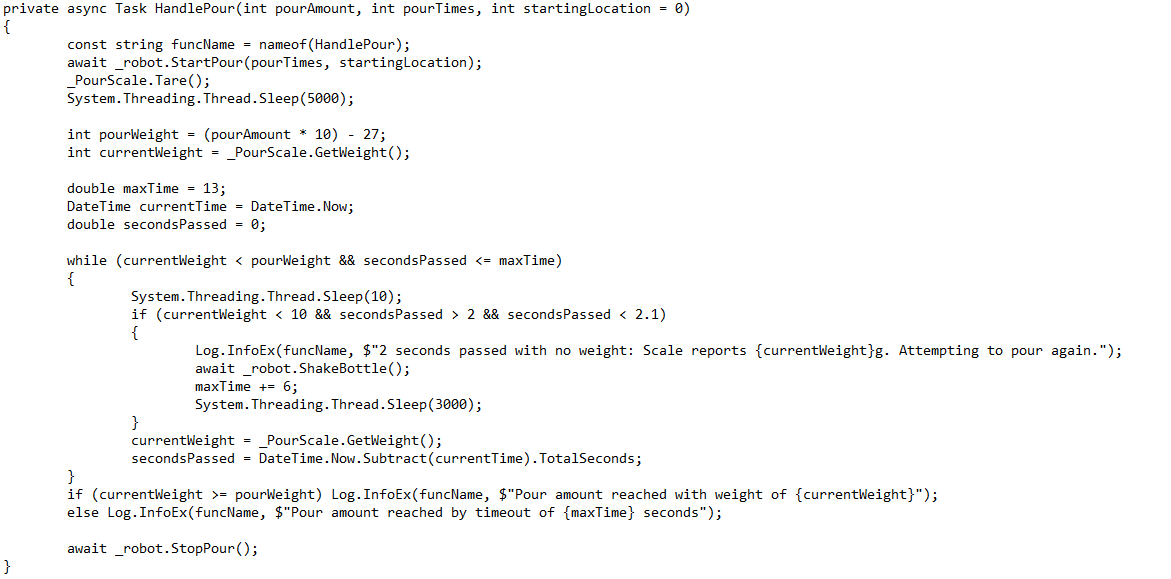
\includegraphics[scale=0.6]{img/HandlePour.png}
\end{center}
\caption{HandlePour-funktio}
\label{fig:HandlePour}
\end{figure}

\lstset{style=sharpc}
\lstinputlisting[label={prog:HandlePour}, caption={HandlePour-funktio}]{code/handlePour.cs}

HandlePour kutsuu ensin RobotCellLayerin funktiota StartPour. RobotCellLayer vastaa robotin kanssa kommunikoinnista. StartPour kutsuu robotin jobia, joka on tällä hetkellä nimellä NEWPOUR.

\begin{figure}[h]
\begin{center}
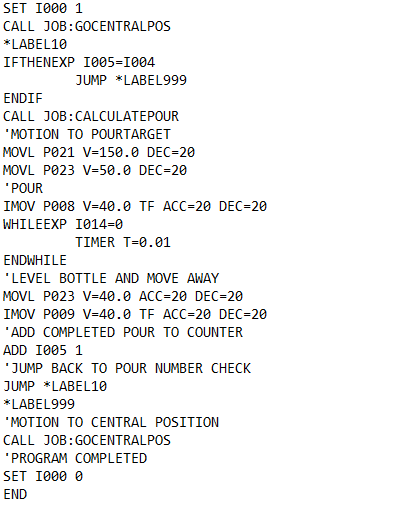
\includegraphics[scale=0.8]{img/NEWPOUR.png}
\end{center}
\caption{NEWPOUR-robottijobi}
\label{fig:NEWPOUR}
\end{figure}

NEWPOUR-job on robotin liikkeiltään hyvin samantapainen kuin kappaleessa \ref{ch:vanha_kaato} esitetty POURDRINKS. Aluksi se määrittää kaadettavan mukin sijainnin CALCULATEPOUR-jobilla. Sitten robottia käsketään siirtymään kaatopisteelle ja robotti kallistaa pulloa aloittaen kaadon. Uutta on kuitenkin se, että robotti jää while-loopin ansiosta odottamaan, että muuttuja I014 on 0. I014 on nimetty robotissa nimellä ``pour ready signal''.

HandlePour-funktio laskee halutun painon kertomalla halutun nesteen tilavuuden, joka on senttilitroina, kymmenellä, jolloin saadaan haluttu massa grammoina. Tästä vähennetään vielä vakio 27. Tämä vakio on määritetty testaamalla ja se kuvaa sitä viivettä, joka kestää siitä kun vaaka tunnistaa massan olevan sopiva, siihen kun nestettä ei enää tule ollenkaan mukiin.

Funktiossa on myös määritelty vakio maxTime, joka on 13 sekuntia. Tämä vakio on määritetty sen perusteella, että kappaleessa \ref{ch:vanha_kaato} esitellyn kaatoajan funktion mukaan saadaan 13 sekunnin kaadolla n. 25 senttilitraa juomaa. Drinkkirobotin tarjoilussa käyttämät lasit ovat tavallisesti hieman yli 25 senttilitraa tilavuudeltaan. Tätä maxTime-vakiota käytetään siihen, ettei mahdollisessa vaa'an virhetilanteessa juomaa kaadeta siten, että se läikkyisi lasista yli.

Fuktiossa on while-looppi, joka odottaa joka iteraatiolla kymmenen millisekuntia, kysyy uutta vaa'an havaitsemaa massaa, ja sen jälkeen tarkistaa onko havaittu massa yhä pienempi kuin haluttu massa. Samalla looppi tarkistaa, ettei kaato ole kestänyt yli maxTime-vakiossa määriteltyä aikaa. Kun while-loopista on tultu ulos, niin tulostetaan konsoliin tieto saavutetusta massasta tai mahdollisesti ajasta ja kutsutaan RobotCellLayerin funktiota StopPour.

StopPour-funktion tehtävänä on ainoastaan muuttaa robotin muuttuja I014, eli ``pour ready signal'' arvoon yksi. Tällöin robotin jobi tulee omasta while-loopistaan ulos, jolloin robotti suoristaa pullon ja näin lopettaa kaadon.


\section{Uuden kaatoratkaisun analysointi}
\label{ch:uuden_analysointi}
Logiikka laskee halutun juoman massan kaavalla
\begin{align}
    \mathrm{pourWeight} = \mathrm{pourAmount} \cdot 10 - 27 \mathrm{,}
\end{align}
eli halutusta massasta vähennetään vaa'an hitautta kuvaava vakio 27. Hitaus johtuu muun muassa tietoliikenneyhteyden hitaudesta ja silmukoiden sisällä olevista odotusajoista. Esimerkiksi robotin tehtäväohjelmassa olevan timer-komennon tai logiikassa olevan sleep-komennon arvoa nostamalla tuo vakio 27 kasvaisi. Tämä hitaus tarkoittaa sitä, että pullon suoristusliikkeen aikana tapahtuviin muuttujiin ei pystytä enää vaa'an avulla vaikuttamaan. Käytännössä siis 27 grammaa juomaa kaatuu vielä sen jälkeen, kun logiikka havaitsee juomaa olevan tarpeeksi. Tämä on kuitenkin vain pieni osa koko kaatoliikettä. Esimerkiksi kaatonokan vaihtaminen sellaiseen kaatonokkaan, jossa virtausnopeus on eri, aiheuttaa sen, että tuo vakio muuttuu hieman.

Painoanturin tarkkuutta testattiin vertailemalla vaa'an antamia tuloksia tavallisen keittiövaa'an näyttämän painon kanssa. Kaikissa tapauksissa painoanturin ja keittiövaa'an tulokset erosivat maksimissaan yhdellä grammalla toisistaan. Vaaka osoittaa hieman liian suuria lukemia johtuen siitä, että juomavirta osuu lasin pohjaan ja osumisen impulssi aiheuttaa voiman. Kuten Fox ja McDonald \cite[s.197-198]{Fox2011} johtivat, Newtonin II laista saadaan voima, joka aiheutuu nestevirtauksen osumisesta pintaan. Tämän voiman suuruus yhteen koordinaattisuuntaan on
\begin{align}
    F_z = \rho Q \delta v_z \mathrm{,}
\end{align}
jossa $\rho$ on nesteen tiheys, $Q$ on virtausnopeus ja $\Delta v_z$ on nesteen nopeuden muutos tuohon koordinaattisuuntaan. Koska juomaa kaadetaan niin matalalta, sen nopeus ei ehdi missään kohtaan olemaan kovin suuri. Lisäksi virtausnopeus on varsinkin kaatonokalla kaadettaessa melko pieni, luokkaa 20 millilitraa sekunnissa. Tämän takia nesteen virtauksesta vaakaan aiheutuva
voima on hyvin pieni ja se vastaa vaa'an lukemassa grammojen epätarkkuutta. Tätä kuitenkin kompensoi yllä kuvattu vakio 27.

HandlePour-funktio taaraa vaa'an ennen jokaista kaatoa. Tämän ansiosta useamman komponentin juomasekoituksia on mahdollista kaataa tällä systeemillä. Funktiossa oleva currentWeight on siis mukiin tullut paino sen jälkeen, kun kyseisen komponentin kaato on aloitettu. Taaraus mahdollistaa myös mukitelineen pitämisen vaa'an päällä ilman että sen massaa erikseen vähennetään saadusta painosta. Mukiteline auttaa siihen, ettei muki liikahda juomavirran vaikutuksesta. Samoin voitaisiin myös käyttää erilaisia, eri painoisia mukeja ilman että se vaikuttaa kaatoihin. Kuvassa \ref{fig:kaato} näkyy robotti kaatamassa vaa'an päällä olevaan mukiin, joka on mukitelineessä.

\begin{figure}[h]
\begin{center}
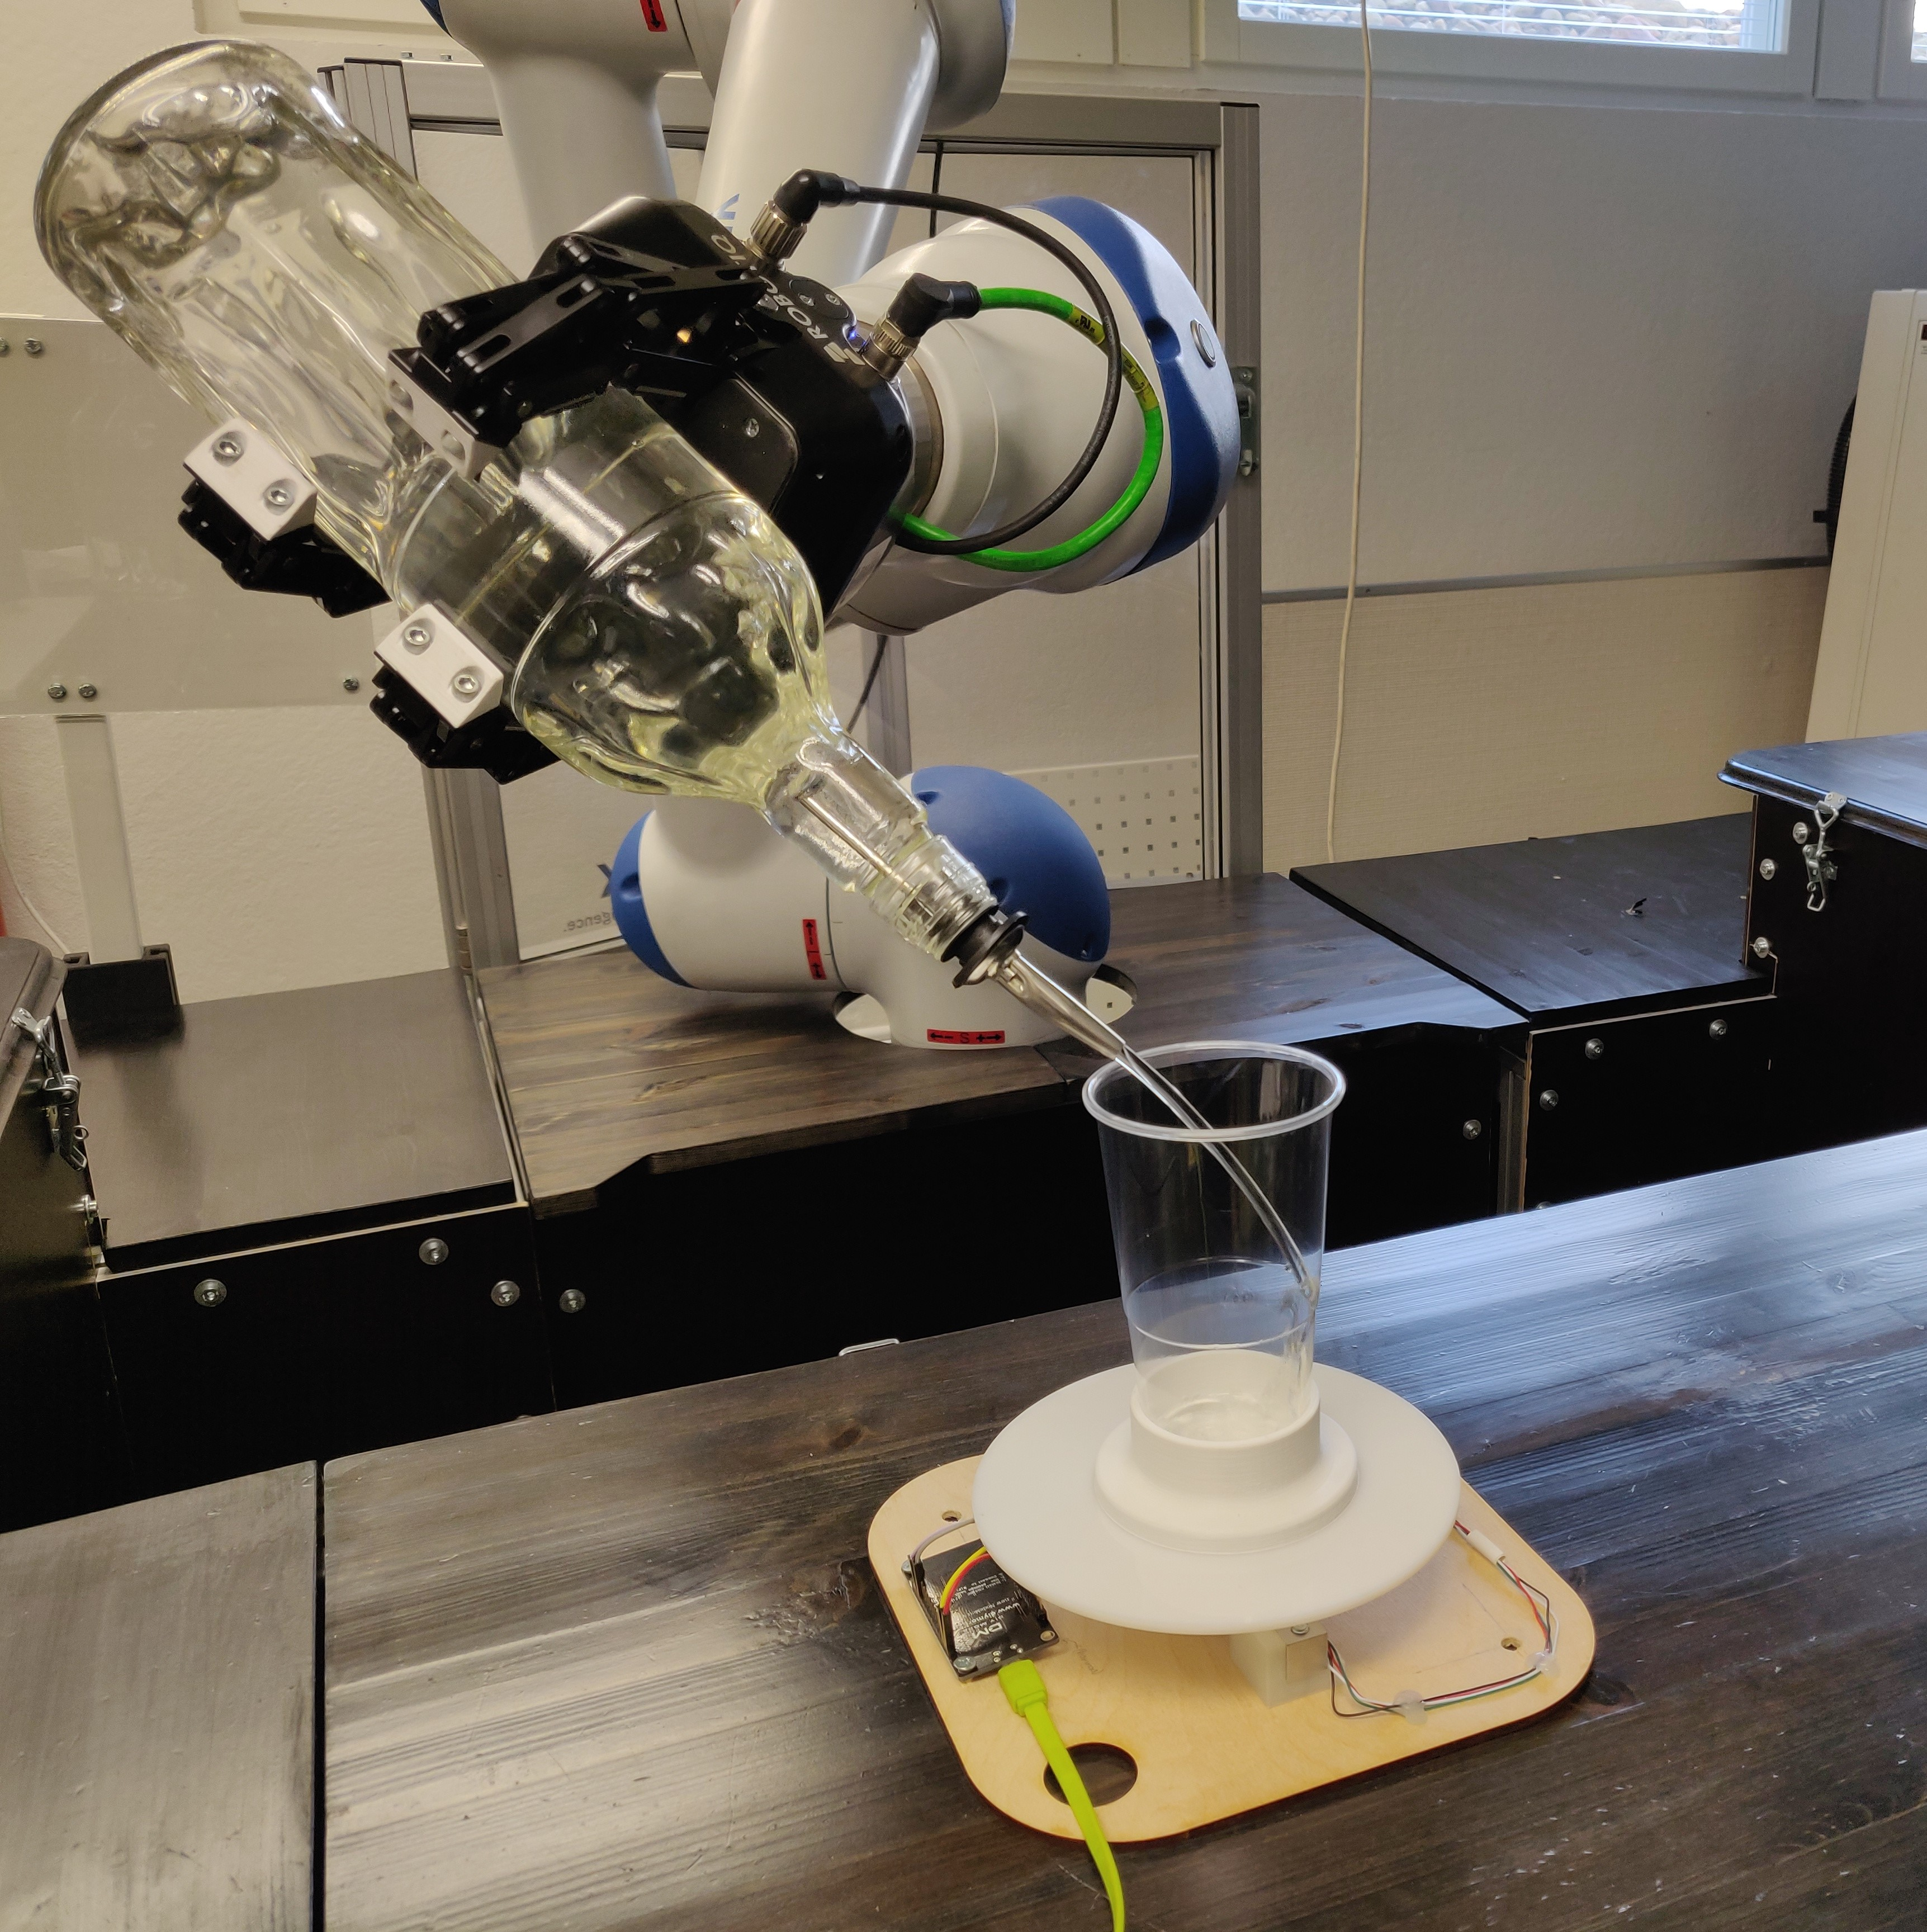
\includegraphics[scale=0.1]{img/kaato.jpg}
\end{center}
\caption{Robotti kaatoasennossa kaatamassa vaa'an päällä olevaan mukiin}
\label{fig:kaato}
\end{figure}

Uusi kaatosysteemi ei tällaisenaan mahdollista alle kolmen senttilitran kaatoja robotilla. Tämä johtuu siitä, että pelkkä kallistus- ja suoristusliikkeen aikana pullosta virtaava juoma on tilavuudeltaan noin kolme senttilitraa, vaikka robotti ei pysyisi kaatoasennossa paikallaan. Pienempiä kaatoja olisi luultavasti mahdollista saada muokkaamalla kaatoasennon kulmaa pienemmäksi. Alaluvussa \ref{ch:vanhan_ongelmat} luetellut lakisääteiset alkoholijuomien perusannokset eivät kuitenkaan vaadi alle neljän senttilitran kaatoja. Tämän takia pienten kaatojen mahdollisuutta ei lopulta ole tässäkään työssä toteutettu.


\chapter{Vertailu}
\label{ch:vertailu}

\section{Vanhan ja uuden kaatoratkaisun vertailu}
\label{ch:vanhan_ja_uuden_vertailu}
Työssä tutkittiin sekä vanhan että uuden kaatoratkaisun pohjalta saatuja tuloksia kaatojen määrissä, jotta niitä voitaisiin vertailla. Kaatoja tehtiin 4cl, 10cl, 16cl ja 20cl kokoisilla tilauksilla. Samalla jokaisen kaadon välissä punnittiin pullossa jäljellä oleva neste, jotta voidaan huomioida sen vaikutus kaadon määrään. Ideaalisesti pullossa olevan nesteen määrä ei vaikuttaisi kaadon määrään.

\begin{figure}[h]
\begin{center}
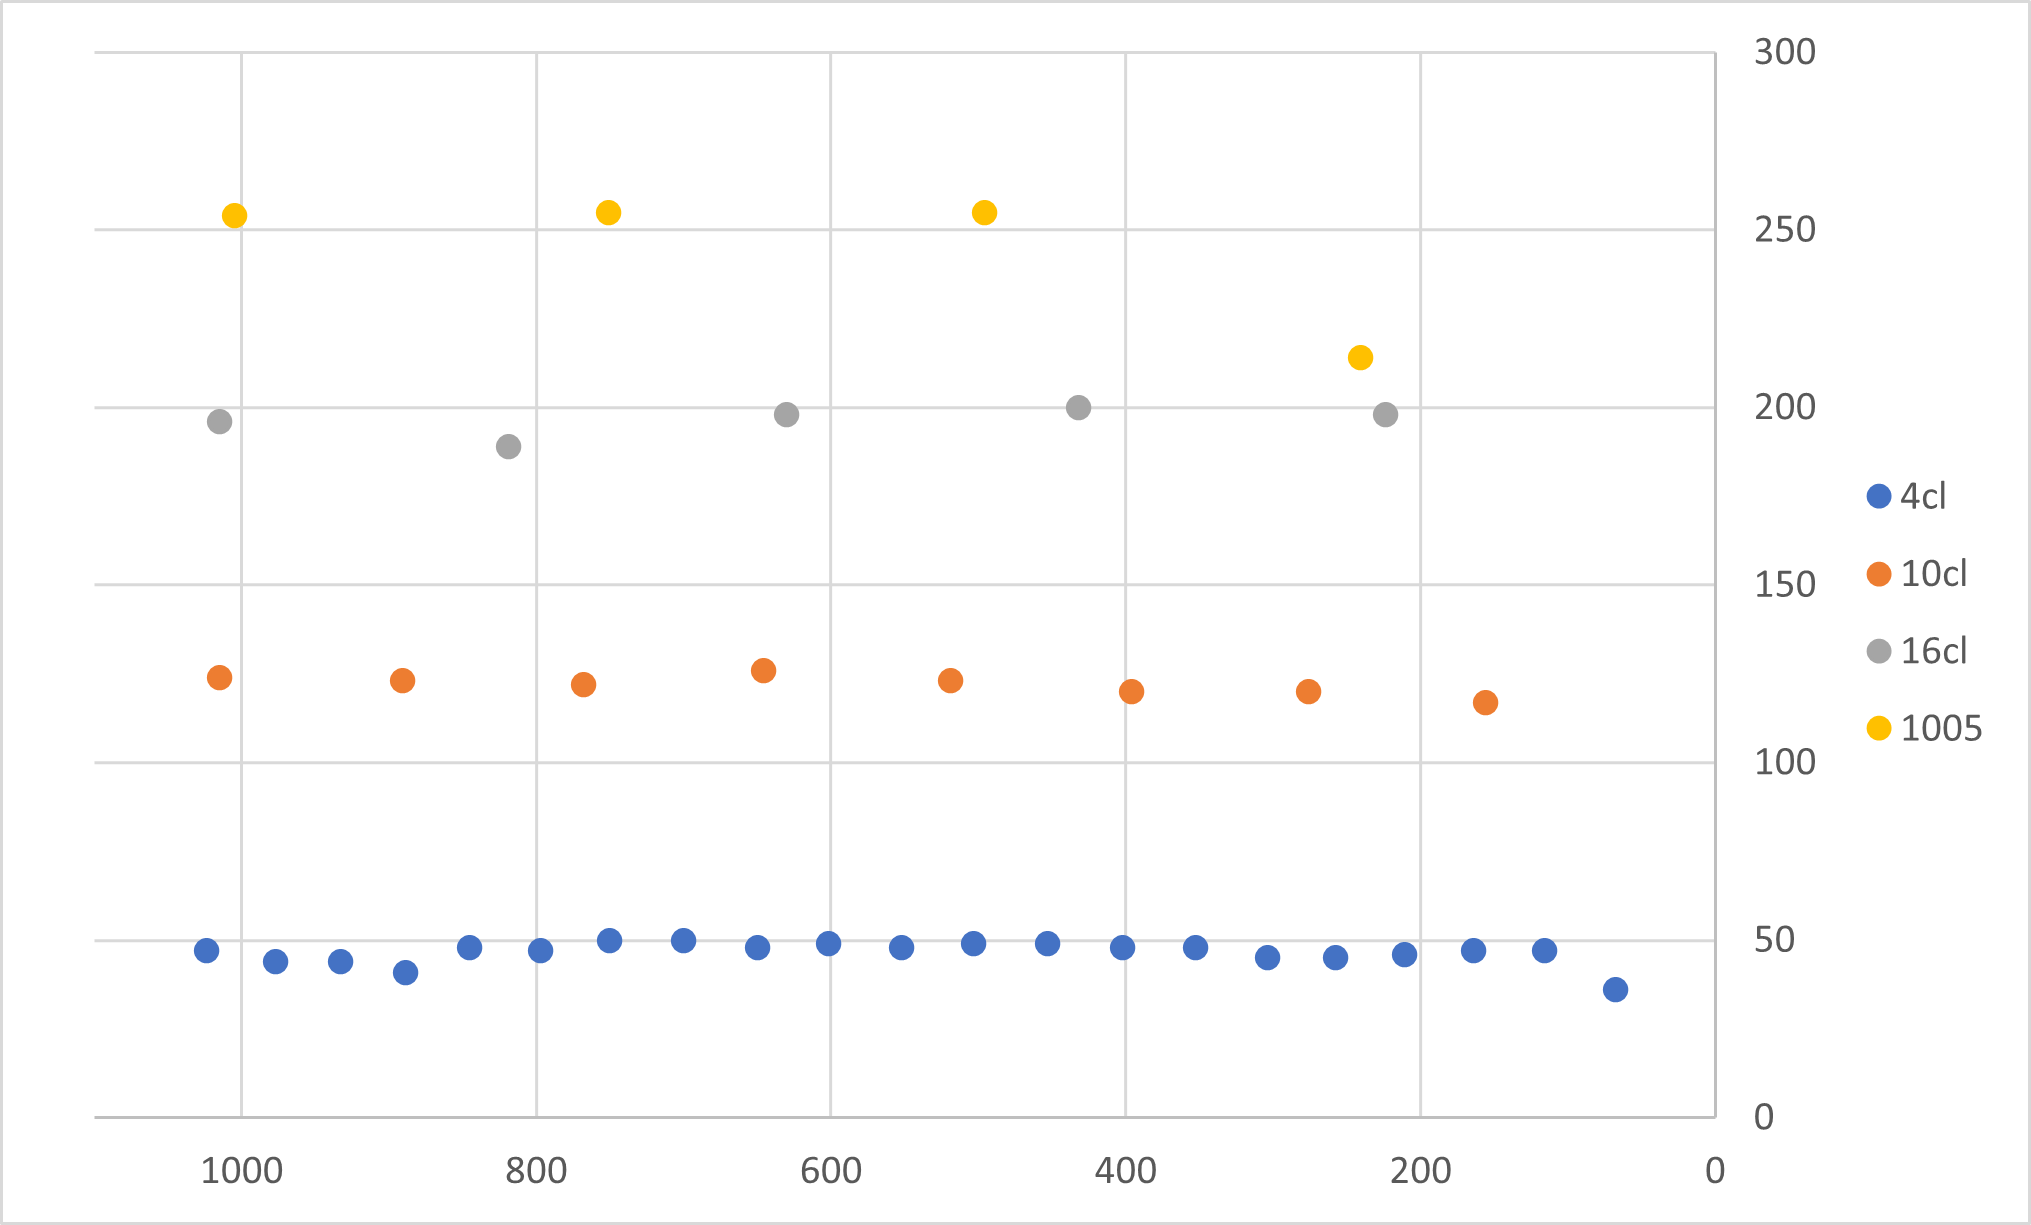
\includegraphics[scale=0.6]{img/kaadot_vanha_kesken.png}
\end{center}
\caption{Vanhalla kaatoratkaisulla saadut tulokset}
\label{fig:kaadot_vanha}
\end{figure}

Kuten yllä olevasta vanhan kaatoratkaisun tulosten kuvaajasta huomataan, varianssia oli kohtalaisen paljon. Saadut juomamäärät laseissa eivät olleet tasaisia, vaan joka kaadolla ne muuttuivat hieman. Esimerkiksi 4cl tilauksessa suurin saatu juomamäärä oli noin 50 grammaa ja pienin n. 36 grammaa. 20cl tilauksessa suurin saatu juomamäärä oli noin 255 grammaa ja pienin n. 214 grammaa. Näiden välinen ero on huomattava, varsinkin kun tarkastellaan eron prosentuaalista osuutta halutusta juomamäärästä.

Kuvaajassa olevista tuloksista saadaan myös vahvistus väitteelle, että pullossa jäljellä oleva juomamäärä vaikuttaa saatuun juoman määrään. Usealla kaatomäärällä mukiin saatu määrä vaihtelee ensin satunnaisesti tietyllä välillä, mutta käyrän loppupää kääntyy alaspäin. Tästä voidaan päätellä, että

Sen lisäksi, että saadut juomamäärät vaihtelevat keskenään paljon ja pullossa oleva juomamäärä vaikuttaa saadun juoman määrään, kaatomäärät ovat myös keskimäärin liian suuria. Koska jokaisella kaatomäärällä juomaa on tullut liikaa suhteessa tilattuun määrään, voidaan päätellä että vanhan funktion kulmakerroin on ollut liian suuri.

Seuraavaksi alla on esitetty kuvaajassa uuden kaatoratkaisun tulokset, jälleen 4cl, 10cl, 16cl ja 20cl kokoisilla tilauksilla.


\chapter{Yhteenveto}
\label{ch:yhteenveto}
Työn tavoitteena oli kehittää Pullonkaula ry:n Drinkkirobotti\hyp{}sovellukselle tarkempi tapa kaataa juomia siten, että tuloksena saadaan oikea tilavuus juomaa. Työssä annettiin ensin yleiskuva Drinkkirobotti\hyp{}sovelluksesta ja sen rakenteesta ja ohjelmistoarkkitehtuurista. Sitten käsiteltiin aikaisemmin käytössä ollutta tapaa juomien määrän mittaamiseen ja kerrottiin, minkälaisia ongelmia sen käytössä on ollut. Juomien kaadossa ongelmia aiheuttaa mm. epälineaarisuus virtaavan juoman määrässä sen suhteen, miten paljon pullossa on juomaa jäljellä. Pahimmassa tapauksessa juomanokan korvausilmaputken tukkeutuminen aiheuttaa pulloon jäävän alipaineen takia sen, että asiakkaan lasi jäi lähes tyhjäksi. Tälle tapaukselle ei voitu vanhalla kaatotavalla muuta kuin tilata uusi juoma. Työssä perusteltiin, miksi kaadon tarkkuus on tärkeää, ja näihin ongelmiin pyrittiin löytämään ratkaisu työssä kehitetyllä uudella kaatotavalla.

Välissä kartoitettiin viime vuosina tehtyjä tutkimuksia aiheesta. Useampia eri ratkaisuja juomien kaadon tarkentamiseksi löydettiin. Näissä ratkaisuissa on käytetty robotin nivelen voima-anturia, haptista etäohjainta, kamerakuvaa tai jopa äänidataa kaadoista, sekä näiden yhdistelmiä. Näiden yhteydessä käytettiin monessa ratkaisussa koneoppimista esimerkiksi kamera- tai äänidatan prosessoinnissa ja niiden yhdistämisssä kaadettuun juomamäärään.

Tässä työssä päädyttiin ratkaisuun, jossa kaadon kohteena olevan juomalasin alle laitetaan vaaka. Tämän ratkaisun valintaan vaikutti sen helppous, sillä robottisolussa oli jo käytössä vaaka, jota pystyttiin hyödyntämään työssä. Lisäksi tällaista tapaa pystyisi helposti käyttämään tavallisissa robottisolussa, kunhan vain vaakaan saadaan yhteys esimerkiksi robottia ohjaavan logiikan kautta. Se ei siis aseta suuria vaatimuksia robottisolulle, eikä vaadi kallista laitteistoa. Uusi kaatotapa toimii siten, että robotin logiikka pyytää vaa'alta jatkuvasti kaadon aikana tuloksia painosta, ja käskee robottia lopettamaan kaadon, kun juomaa on tarpeeksi.

Uudella kaatotavalla päästiin hyviin tuloksiin. Kaikki testatut juomamäärät vaihtelivat korkeintaan yhdellä grammalla. Lisäksi saatiin ratkaistua kaatonokan korvausilmaputken tukkiutumiseen liittyvä ongelma, joka johti virtauksen estymisen takia siihen, että asiakkaan lasi jäi lähes tyhjäksi. Tämä ongelma ratkaistiin siten, että logiikka havaitsee jos juomaa ei virtaa lasiin ja käskee robottia tekemään uuden kaatoliikkeen. Uuden kaatotavan heikkous on se, että kaadon jälkeen pullon suoristuksen aikana virtaavaan juomamäärään ei pystytä vaikuttamaan. Pienten, alle kolmen senttilitran kokoisia kaatoja ei ole myöskään mahdollista tehdä. Näiden heikkouksien ratkaisemiseksi olisi mahdollista tehdä kaatokulman säätö, ja se voisi olla tulevaisuuden kehityskohde Drinkkirobotti\hyp{}sovellukseen.


%%%%% Bibliography/references.

% Print the bibliography according to the
% information in ./tex/references.bib
% and the in-line citations used in the body
% of the thesis.
% \emergencystretch=2em
\printbibliography[heading=bibintoc]

%%%%% Appendices.

% Use only if it clarifies the structure of
% the document. Remember to introduce each
% appendix.

%\begin{appendices}
%\end{appendices}

\end{document}
